\section{Présentation}



\subsection{Contexte d'enseignement}



Lauréat du concours du CAPES de Numérique et Sciences Informatique (NSI), je suis  cette année professeur stagiaire. Préalablement fonctionnaire de l'éducation nationale en tant que professeur en lycée professionnel (PLP) de mathématiques, sciences-physiques et chimiques, je bénéficie du statut de professeur stagiaires à \emph{temps complet}. C'est l'occasion pour moi de produire cet écrit réflexif qui se propose de décrire un dispositif pensé et mis en œuvre durant cette année dans la cadre du master 2 Métiers de l'Enseignent, de l'Éducation et de la Formation (MEEF).

En effet, cette année est pour moi très particulière puisque, outre la découverte d'une discipline nouvelle à enseigner, j'assiste en parallèle à certains cours du M2 MEEF avec des professeurs stagiaires à \emph{temps partiel} de NSI et sciences de l'ingénieur (SI). Bénéficiant d'une validation des acquis pour certaines unités d'enseignement (UE) ainsi que d'une dispense de cours, je travaille néanmoins sur la validation de l'UE 2, accompagné pour cela par Jean-François Herold.

J'enseigne à 18 heures dans le lycée Simone Veil de Marseille (13~013). Cet établissement de 850 élèves accueille les élèves de la seconde au BTS et admet une section professionnel.

Mon service est partagé entre :

\begin{description}
    \item[8 heures] d'enseignement de sciences numériques et technologie (SNT) auprès de quatre classes de seconde et
    \item[10 heures] d'enseignement de NSI auprès d'élèves de première et de terminale.
\end{description}

L'enseignement de NSI est un \emph{enseignement de spécialité} qui a vu le jour avec la \emph{réforme du baccalauréat général et technologique et du lycée} de 2018. Cette réforme, après une succession d'évolutions, de modification et d'ajustements, propose actuellement et jusqu'à nouvel ordre aux élèves de fin de seconde de choisir trois enseignements de spécialités parmi l'ensemble des enseignements disponibles sur leur secteur d'affectation. En fin de première, ces derniers conservent deux enseignements, qui seront évalués au baccalauréat par des épreuves ponctuelles, et arrêtent leur troisième spécialité qui sera évaluée au baccalauréat par le contrôle continu.
\\
En fin de seconde, lors du choix des spécialités libre a lui (et à sa famille) de reproduire les menus traditionnels tels que :

\begin{itemize}
    \item pôle scientifique type S avec les spécialités mathématiques, physiques et sciences et vie de la terre (SVT)
    \item pôle littéraire type L avec humanité, littérature et philosophie (HLP), langue, littératures et cultures étrangères (LLCE)
    \item pole économique et social type ES avec histoire géographie, géopolitique et sciences politiques (HGGSP), sciences économiques et sociales (SES).
\end{itemize}

Néanmoins d'autres voies sont possibles et désormais l'éducation physique et sportive (EPS), les sciences de l'ingénieur (SI), la musique, l'audiovisuel ou les sciences informatiques font leur apparition auprès des spécialités typées plus traditionnelles.



\subsection{Trois constats}



\paragraph{Des élèves qui ne se connaissent pas}
%
En tant qu'enseignants de spécialité, je constate que je me retrouve face à un groupe d'élèves dont les seuls moments partagés se font dans notre cours. 
\\
En effet, cette individualisation du choix couplée à la richesse de l'offre engendre une très grande variété de couplages sur les cohortes d'élèves de première et de terminale. Par exemple sur mon établissement qui propose 9 enseignements de spécialités, pas moins de 84 combinaisons différentes sont possibles. Sur ces deux niveaux, il n'existe donc plus de classe aux spécialités homogènes. C'est-à-dire qu'il n'existe plus de classes dont tous les élèves suivent les mêmes enseignements de spécialité. Les classes de spécialité sont donc devenues des \emph{groupes} de spécialités, et la très grande majorité de ces groupes sont constitués d'élèves provenant de classes différentes.
\\
Ce morcellement des classes implique que les élèves se retrouvant dans chaque groupe de spécialité se connaissent beaucoup moins. Ils ne se côtoient ensemble que pendant les heures consacrées à chaque enseignement de spécialité. Le parcours de chaque élève est donc fortement individualisé et les groupes de spécialité sont structurellement d'une constitution autre que celle de la classe entière ou de ses demi-groupes. Il me semble que le fonctionnement structurel induit par la \emph{réforme du baccalauréat général et technologique et du lycée} engendre une école cloisonnant l'individu plutôt qu'une école comme levier de promotion du collectif. 


\paragraph{Nécessité d'une pédagogie différenciée}
%
En tant qu'enseignant, nous sommes face au constat que notre enseignement doit être différencié. Certes, c'est un lieu commun pour les institutions et le monde de la recherche, mais concrètement, face aux élèves, la réalité est implacable : les élèves sont tous différents. Par leurs expériences vécues, leurs façons de vivre la classe, leurs intégrations dans le groupe ou encore leurs sensibilités. Il ne peux donc pas en être autrement sur leurs besoins ou leurs façons d'apprendre.
\\
Cette différenciation est relativement aisée à penser en enseignement d'informatiques. Les environnements de travail, qu'ils soient matériels ou numériques, aident à la rendre opérationnelle. Muni d'un ordinateur et d'un espace de travail, il est facile de proposer des activités adaptées aux besoins de chacun. C'est un gros travail de logistique et de création, mais ça ne pose pas de grosses difficultés conceptuelles.


\paragraph{Importance du socio-constructivisme}
%
Enfin, je suis un enseignant convaincu de l'importance pour l'apprentissage de la dimension sociale.  Pour un enseignant, il est moins efficace de transmettre un savoir que de le faire se construire par l'apprenant. Cette dimension constructiviste peut prendre plusieurs formes comme une situation problème particulièrement bien sentie et adaptée à l'élève ou encore comme une verbalisation ou une reformulation dans un contexte proche.
\\
Je trouve l'approche par situations problèmes délicate à mettre en œuvre. Il faut une disponibilité de l'élèves au moment de la rencontre. Il est aussi nécessaire de prendre en compte la zone proximale de développement de l'élève pour rendre la tâche tout à la fois accessible mais pas trop. Cette symbiose entre l'apprenant, le savoir et la situation me paraît trop difficile à penser en amont. 
\\
En revanche, le constructivisme peut aussi trouver sa réalisation par l'approche sociale. Cet aspect met en avant les besoins fondamentaux humains que sont l'échange, le partage, l'empathie ou encore le vivre ensemble. Le socio-constructivisme défend qu'un savoir se construit d'autant mieux s'il émerge d'interactions sociales. Je trouve cette approche pertinente pour plusieurs raisons. D'une part, en étant bien menée, l'apprenant se sent mieux dans un groupe qui devient de plus en plus bienveillant. D'autres part, en trouvant des dispositifs adaptés ne prétendant pas tout anticiper, cette démarche, plus aisée à mettre en œuvre, s'appuie sur la diversité des élèves, de leurs échanges et de leurs interactions.


\paragraph{Face à la contradiction}
%
Avec ma nouvelle discipline à enseigner et dans ce contexte de groupe de spécialité, j'ai été troublé par le fait que les élèves ne se connaissent pas. Cette individualisation des parcours et ce cloisonnement m'apparaît clairement contradictoire avec le socio-constructivisme si important pour l'apprentissage. Si les interactions entres les élèves sont minimales, il y a alors absence d'intérêt, d'échange ou de partage entre eux.
%
C'est pourquoi pendant l'année il m'est apparu primordial de favoriser les interactions entre les élèves.Il m'était nécessaire de mettre en œuvre un dispositif de pédagogie différenciée qui puisse promouvoir le collectif.



\section{Méthode Jigsaw}

\subsection{Description de la méthode}


Parmi les différentes méthodologie proposée de pédagogie différenciée, je me suis tourné vers une pédagogie de \emph{tutorat bidirectionnel}. 
\\
L'idée de tutorat est de créer des groupes d'élèves intégrant deux rôles asymétriques : l'élève \emph{tuteur}, qui transmet un savoir, et l'élève \emph{apprenant}, qui découvre le savoir transmis par son camarade.
% 
Mais cette asymétrie possède le risque de la stigmatisation. Qu'il soit étiqueté par ses camarades \emph{bon} ou \emph{mauvais}, la classe ne doit pas être le lieu de ses tensions. C'est pourquoi le dispositif de tutorat doit pour moi permettre à tous les élèves de tenir chacun des deux rôles. C'est cet aspect là du tutorat que l'on qualifie de \emph{bidirectionnel}.
\\
J'ai donc imaginé un dispositif qui ressemble beaucoup à la méthode \emph{jigsaw} apparue aux États-Unis dans les années 1970 pour faire face à la déségrégation.

L'idée est de partitionner une notion globale à enseigner en savoirs distincts puis d'organiser la séance en deux moments aux objectifs différents :

\begin{description}
    \item[moment de l'appropriation] Dans un premier temps, des groupes d'élèves sont constitués et chaque groupe a pour objectif de s'approprier un savoir. Chaque groupe possède un savoir différent à étudier. Durant ce moment, tous les élèves prennent connaissance au sein de leur groupe d'expert d'un savoir dont ils seront les tuteurs.
    \item[moment de la transmission] Dans un deuxième temps, on répartit tous les élèves dans d'autres groupes de façon à séparer les tuteurs. Les nouveaux groupes créés doivent posséder au moins un tuteur de chacun des savoirs concerné. Durant ce moment, chaque élève doit s'approprier l'ensemble des savoirs ce qui oblige chaque tuteur à exposer, expliquer et faire comprendre le savoir dont il est le garant.
\end{description}



\subsection{Mise en place du dispositif}



Comme on peut le constater, chaque élèves est à la fois tuteur d'un savoir et apprenant de l'ensemble des autres savoirs.

Ce dispositif :

\begin{itemize}
    \item permet une absence totale de stigmatisation entres élèves et 
    \item favorise un échange très fort entres élèves centré sur le savoir.
\end{itemize}

Lors de la mise en œuvre d'un tel dispositif, puisque le moment d'appropriation nécessite une grande autonomie des élèves, il est indispensable de créer ces premiers groupes de façon différenciées. Il faut des groupes d'experts en phase avec le savoir à s'approprier, et pour cela il faut que les élèves d'un même groupe aient des zones proximales de développement (ZPD) proches et sécantes entres elles.
\\
Un avantage de cette différenciation en amont des élèves est de se faciliter la répartition des savoirs entres les groupes puisqu'on s'autorise à avoir des savoirs de niveaux et de difficultés différentes.

C'est pourquoi, une première étape d'évaluation des élèves est indispensable. Lors de ce moment de la différenciation, je me suis efforcé de créer des groupes de niveaux en lien avec les prérequis nécessaires lors des moments suivants.

La méthodologie réalisée a donc été organisée en trois étapes :

\begin{description}
    \item[étape (a)] moment de la différenciation pour créer des groupes de niveaux,
    \item[étape (b)] moment de l'appropriation pour former les futurs tuteurs, par groupe de niveau, sur les savoirs à transmettre,
    \item[étape (c)] moment de la transmission pour que chaque élève transmette au sein de son groupe son savoir.
\end{description}


\begin{center}
    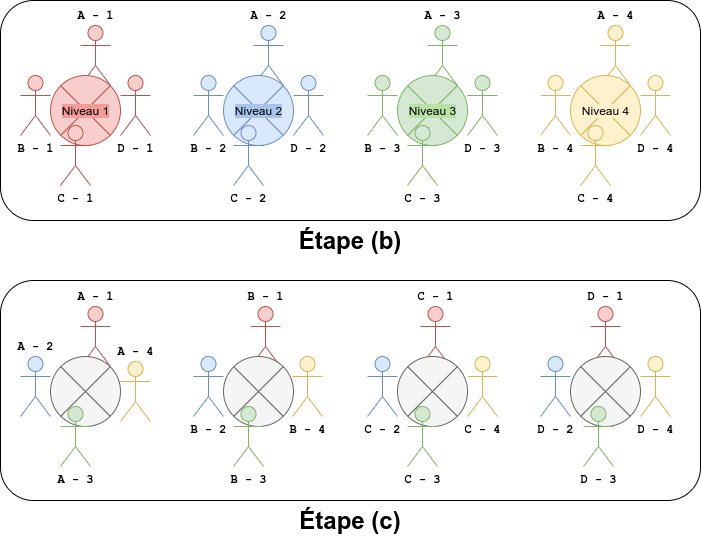
\includegraphics[width=0.75\linewidth]{res/diagramme.drawio.png}
\end{center}



\section{Première expérimentation}


J'ai procédé à ma première expérimentation au mois de mars. La notion globale travaillée concerne \emph{les types de base en informatique et la représentation des données en machine}.



\subsection{3 moments de la séances}



\paragraph{Moment de la différentiation}
%
J'ai listé les prérequis nécessaires au savoir global à enseigner lors de la séance tutorée. J'ai organisé ces prérequis en tâches puis j'ai organisé une première séance abordant chacune de ces tâches. À l'issue de cette séance, j'ai procédé à une évaluation des élèves pour créer des groupes de niveaux.
%
Pour faciliter la collecte des données et l'analyse à posteriori, j'ai décidé de travailler avec un outil dédié à l'enseignement en ligne : Moodle. J'ai proposé aux élèves une série de tests évaluant chacune des tâches identifiées.

Afin de ne pas pénaliser les élèves les plus lents et pour valoriser l'apprentissage des prérequis, j'ai autorisé pour chaque test un nombre illimité de tentatives. Mais afin de ne pas biaiser les résultats par des \emph{copier/coller}, j'ai mis en place des tests basés sur des valeurs aléatoires. C'est donc bien la méthode qui doit être correcte et non pas le résultat saisi ou coché.
%
Puisque le travail est en ligne, il a même été possible de demander aux élèves de finir le travail sur leurs temps personnels, en dehors de la classe. J'ai ainsi été conforté dans l'idée que les prérequis étaient assimilés.

À l'issue de cette séance, j'ai donc eu en ma possession une feuille de calcul indiquant pour chaque tâche, le niveau de réussite, le nombre de tentative et le temps passé par chaque élève.
%
Pour le moment de l'appropriation, j'ai besoin d'avoir des groupes homogènes. J'ai donc procédé à un classement des élèves par notes.
\\
Mais j'ai aussi voulu mettre en avant les élèves en fonction de leur degré d'autonomie. Pour cela, j'ai aussi pris en compte la durée totale nécessaire à l'achèvement d'une tâche donnée. Ainsi, mon classement final dépend de deux paramètres : le niveau de réussite et la vitesse de réalisation.

Pour chaque élèves, j'ai additionné pour chaque tâche son classement dans la classe et j'ai ainsi obtenu un score pour chaque élève. Plus ce score est petit, mieux l'élève a été classé en moyenne. Ce score m'a permis de créer trois groupes de niveaux nécessaire au moment de l'appropriation.


\paragraph{Moment de l'appropriation}
%
Quelques semaines plus tard, j'ai procédé au moment de l'appropriation. 

J'ai donc organisé les élèves par groupes, sans bien évidemment leur dire que c'était des groupes de niveaux. Chaque groupe a eu une feuille d'activité composée d'un savoir, de quelques exemples et d'une ou deux activités. Entres les groupes d'appropriation, les savoirs sont différents, mais chaque élève d'un même groupe travaille le même savoir.

L'objectif de chaque élève est de s'approprier le savoir, de comprendre les exemples et de savoir faire les activités. Pour cela, les échanges au sein du groupe d'experts sont encouragés ! Lors de la mise en activité, j'ai montré aux élèves la constitution des groupes de transmission à venir en leur indiquant l'objectif global de cette séquence de travail en groupe s'approprier un savoir pour le transmettre plus tard.

Dans les groupes, les élèves on naturellement commencé par lire leur document puis, après un moment de surprise et voyant que je n'intervenais pas, les échanges ont commencé dans les groupes.
\\
Ma posture a été d'intervenir le moins possible pour favoriser le partage et l'échange entre les élèves.


\paragraph{Moment de la transmission}
%
La séance suivante, j'ai mis en place les groupes de transmissions. Une même fiche d'activité est distribuée à chaque groupe. Cette fiche traite de la notion globale qui est constituée de l'ensemble des savoirs de chaque expert. L'objectif pour chaque élève a été clairement formalisé : expliquer aux élèves de son groupe sa notion experte. À la fin, chaque élève doit être capable de traiter seul la notion globale et la séance sera suivie d'un test de connaissance sur la notion globale.



\subsection{Observations et remarques}



\paragraph{Moment de le différentiation}
%
Ce moment a été le plus simple. Les élèves étant habitués à travailler sur Moodle, aucun n'a eu de difficulté pour se mettre au travail. L'activité étant réalisable un nombre illimité de fois, j'ai ajouté la note comme élément de motivation. J'ai indiqué aux élèves qu'il y aurait une note par tâche et que pour chacune d'entres elles, parmi toutes les tentatives réalisées, je garderai la note de celle la mieux réussie. Cet élément de note a été moteur pour inciter les élèves à mieux réussir et à recommencer si besoin leur travail. C'est aussi cet élément qui a fait que le travail a été fini à la maison par la plupart des élèves de la classe.
\\
L'analyse des résultats a été réalisée très simplement au tableur.


\paragraph{Moment de l'appropriation}
%
Pour des raisons externes, ce moment s'est déroulé longtemps après le moment précédent. Les prérequis travaillés préalablement étaient oubliés pour de nombreux élèves. Heureusement le travail en groupe a permis à certains d'expliquer à leurs camarades. Mais il y a eu des groupes qui avaient de gros manques.
\\
Certains élèves absents lors du moment de la différentiation ont été réparti dans les groupes les plus faibles car ils n'avaient pas travaillé les prérequis. Ce manque leur a été préjudiciable dans la phase d'appropriation car certains éléments leur échappaient complètement.
\\
L'absence d'autres élèves lors de ce moment m'a obligé à réorganiser les groupes en direct. À déplacer des élèves et à les changer de \emph{niveau}. Heureusement, et pour éviter la stigmatisation, j'avais préparé un tableau dynamique de groupe organisé en \emph{couleurs} et non en \emph{notes}.
\\
Je me suis rendu compte que j'ai mal évalué la durée de ce moment qui a pris beaucoup plus de temps que je ne le pensais. Je me suis adapté et n'ai pas interrompu le travail et les échanges entres les élèves. J'ai décidé sur le coup de reporter le moment de la transmission à la séance suivante. Ce choix était nécessaire mais a engendré certaines difficultés.
\\
Enfin, le plus gros problème rencontré est lié à mon attitude et à mon rôle durant ce moment : ma posture est à revoir. J'ai en effet décidé d'intervenir le moins possible, mais je me suis rendu compte lors de l'analyse des résultats que certains savoirs n'avaient pas été bien compris. Le problème est que si le savoir est mal interprété par les \emph{experts}, la transmission à venir est de piètre qualité, incomplète, voire erronée. Lors de mes prochaines séances, je pense faire le tour de tous les groupes et ajuster l'appropriation des savoirs.


\paragraph{Moment de la transmission}
%
Ce moment n'ayant pas eu lieu le même jour que le moment précédent, j'ai été confronté à l'absence d'un élève qui était présent précédemment. J'ai du modifier la constitution prévue des groupes. J'ai donc supprimé un groupe et ai réparti les élèves afin de d'avoir l'ensemble des savoirs pour chaque groupe. Cette adaptation a engendré des doublons d'experts.
\\
Par ailleurs, la séance a été interrompu au milieu par le départ de 25\% de mes élèves qui s'étaient inscrit à une présentation avec des intervenants extérieurs. Ce départ que je n'avais pas prévu m'a obligé à revoir la constitution des groupes. Il y a donc des experts qui ont dû expliquer plusieurs fois leurs notions. Il y a aussi des élèves qui, je m'en suis rendu compte après, n'ont pas eu d'explication sur un des savoirs.
\\
Par ailleurs, en voulant favoriser les échanges et en ne voulant pas supplanter le tuteur, je ne me suis rendu compte qu'à posteriori de l'incompréhension et de l'incapacité de certains tuteurs à transmettre une notion qui leur échappait complètement.



\section{Conclusion}



Après cette séquence, j'ai repris l'ensemble des savoirs en classe et les élèves ont retravaillé la notion globale. Ainsi, cette séquence n'est pas une fin en soi et on ne peut pas considérer la notion globale comme traitée suite à un tel dispositif.

Je n'ai pas encore évalué l'efficacité du dispositif au niveau des apprentissages. Néanmoins, je peux déjà apporter une première conclusion. Je trouve que cette expérience partagée par les élèves très enrichissantes pour eux. J'ai vu des élèves se parler et échanger pour la première fois. J'ai apprécier de voir que le savoir était au centre de leur préoccupation à ce moment là et c'était pour moi une expérience très agréable.

La création des fiches en amont a présenté un gros investissement et c'est le principal frein à ce genre de dispositif. En effet, pour chaque savoir il faut créer du contenu de cours, des exemples et des activités. Puis pour la notion globale, il faut créer deux fiches d'activités semblables mais différentes : l'une pour le moment de la transmission, une pour l'évaluation de la notion globale.
\\
Il y a donc beaucoup pour rendre de telles séquence opérationnelle. 

Néanmoins, sous réserve que les apprentissages ne soient pas (trop) dégradés, l'investissement me semble valorisant pour tous. Pour l'enseignant qui découvre une classe autonome et mobilisée et qui offre une expérience du vivre ensemble valorisante. Pour les élèves qui sont amenés à vivre un moment agréable de partage et d'échange centré sur le savoir.